\section{Analysis}
\label{sec:analysis}

\begin{table*}[t]
\caption{Isolating the alias-instead-of-delete rule. Replacing the alias operation by
deletion in the sensitive-and-relevant cell, with everything else held fixed, costs a large
and significant amount wherever the anchor is itself a sensitive value (multi-entity,
single-hop, two-hop) and nothing where it is not (topical variants, no anchor). The
two-hop column is the clearest case: the reference answer is present in the context in
$96.3\%$ of cases under the delete variant, and F1 is nevertheless $0.0000$, because the
account that identifies the record has been removed.}
\label{tab:ablation_alias}
\centering\small
\setlength{\tabcolsep}{6pt}
\begin{tabular}{lrrrr}
\toprule
Benchmark & \textsc{DARK} & delete variant & $\Delta$ & 95\% CI \\
\midrule
extension, all ($2{,}728$)     & 0.4937 & 0.3142 & $+0.1795$ & $[+0.1643,+0.1945]$ \\
\quad multi-entity ($1{,}500$) & ---    & ---    & $+0.3273$ & $[+0.3040,+0.3513]$ \\
\quad needle ($1{,}228$)       & ---    & ---    & $-0.0010$ & $[-0.0105,+0.0086]$ (n.s.) \\
main set ($112$)               & 0.6366 & 0.5205 & $+0.1161$ & $[+0.0446,+0.1875]$ \\
LongBench topical ($300$)      & 0.3516 & 0.3503 & $+0.0013$ & $[-0.0002,+0.0042]$ (n.s.) \\
LongBench single-hop ($300$)   & 0.9607 & 0.1674 & $+0.7933$ & $[+0.7430,+0.8426]$ \\
LongBench two-hop ($300$)      & 0.6733 & 0.0000 & $+0.6733$ & $[+0.6200,+0.7256]$ \\
\bottomrule
\end{tabular}
\end{table*}


\subsection{Why redundancy ordering fails here}

The failure we set out to address is not visible in aggregate F1, so we state it in its own
terms. The question is whether the record carrying the answer survives compression when the
rule that decides is a redundancy ordering. On the $2{,}728$-case extension the redundancy-only
rule retains the answer record in $47.5\%$ of cases ($56.0\%$ multi-entity, $37.2\%$ needle),
protecting the anchor line raises this to $57.6\%$, and routing on the record block reaches
$100\%$.

The two failure rates say different things. Multi-entity survival sits either side of the
budget cut, which is what an uninformative ordering produces: the score does not know which
record the question is about, so it keeps the right one about half the time. Needle survival
is \emph{below} the cut, and there the ordering is worse than uninformative. The answer in a
needle case is a field value that recurs across distractor records, so the record holding it
looks like a typical record and inherits no priority from the score. Protecting the anchor
line repairs this for needle cases---retention rises from $37.2\%$ to $59.9\%$---but the line
it protects is not the line that carries the answer, which is why the repair stops short of
$100\%$ rather than reaching it.

Figure~\ref{fig:survival} breaks the same question down by budget, by source, and by what the
retention is worth. Panel (a) follows the answer record across the budget curve: the two arms
that route on the record block hold it in $100\%$ of the 112 cases from $r=0.50$ upward and in
$56.2\%$ at $r=0.10$, while the two arms that only protect the anchor line stay between
$24.1\%$ and $77.7\%$ across the whole range. Panel (b) sets survival against F1 for the
$2{,}728$-case extension. Survival accounts for a good part of the ordering but not all of it:
the delete variant keeps the answer record in $100\%$ of cases and still scores $0.0000$ on
multi-entity cases, because the record it keeps no longer says which account it belongs to. The
dissociation is not an artefact of the aggregate: panel (c) repeats the comparison within each
of the six sources, and the block-level rule holds the answer in every case of every source
while the redundancy-only rule falls to $16.7\%$ on \arm{toolmem\_raw}. Panel (d) shows what
that retention is worth per source; the one source where the block rule is behind, by
$-0.065$, is the one where the redundancy-only arm retains $83.3\%$ and the two are
effectively tied.

\begin{figure*}[t]
\centering
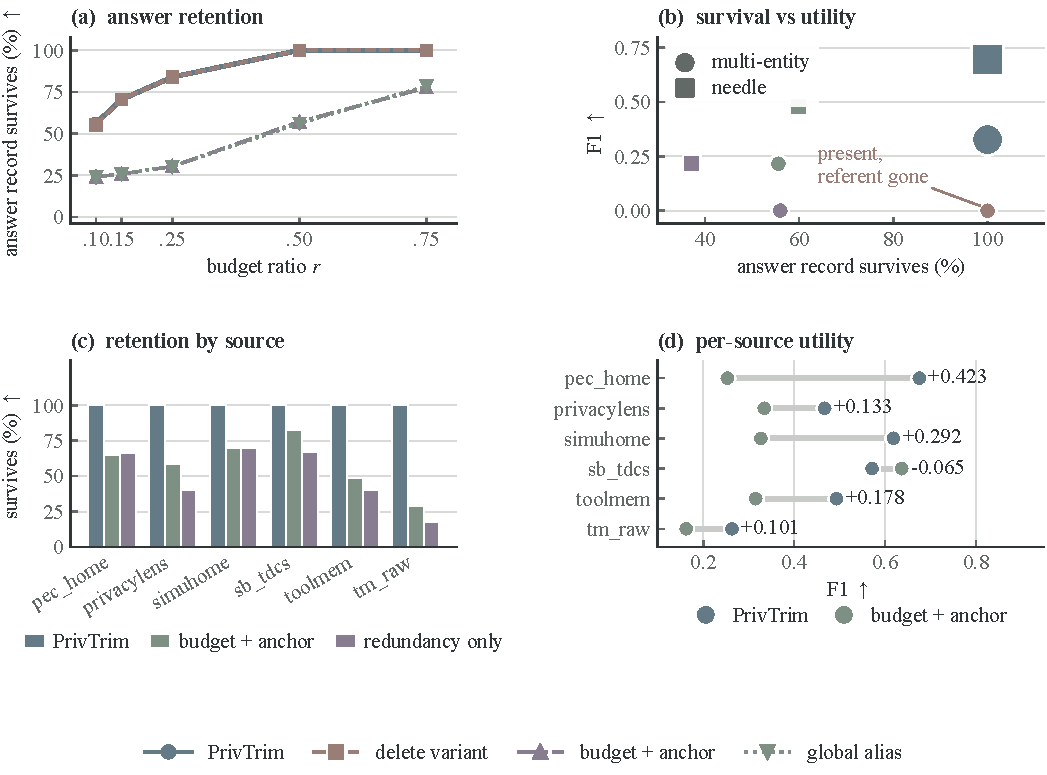
\includegraphics[width=\textwidth]{figures/fig2_diagnostic.pdf}
\caption{Answer retention and what it does not explain. (a) Fraction of the 112 benchmark
cases in which the record carrying the reference answer survives compression, as the budget
varies. \textsc{DARK} and the delete variant coincide almost exactly: the
alias-instead-of-delete rule does not change \emph{which} units survive. (b) Survival against
F1 on the $2{,}728$-case extension; circles are multi-entity cases and squares are needle
cases. The delete variant sits at $100\%$ survival and $0.0000$ F1 on multi-entity cases: the
information is in the prompt and cannot be located. (c) Retention within each source at
$r=0.50$. (d) Per-source F1, \textsc{DARK} against the anchor-protected arm, with the
paired difference printed at each row.}
\label{fig:survival}
\end{figure*}

\subsection{Protecting the anchor line is not enough}

A natural repair forbids dropping units that mention the queried entity. It does not close the
gap, and where it helps it helps for the wrong reason. Overall retention moves from $47.5\%$
to $57.6\%$, but the two families behave differently: multi-entity retention is unchanged
($56.0\%$ to $55.6\%$), while needle retention rises from $37.2\%$ to $59.9\%$. Needle cases
improve because the anchor there is the record identifier, which happens to share the record
with the answer far more often than the account line does. The reason the repair stops short
of $100\%$ is layout: the line carrying the account identifier and the line carrying the
answer are different units in $100\%$ of multi-entity cases and in $65.4\%$ of needle cases.
Preserving the identifier preserves the pointer, not the content.

The repair becomes effective one level up. The excerpt is laid out in record blocks, and the
block containing the anchor mention also contains the answer in $100\%$ of multi-entity cases
and $99.7\%$ of needle cases. Constraining the block instead of the line restores answer
retention to $100\%$ on both families without consulting the answer key. This is the
measurement that motivates the routing rule: the relevant region is a block, not a unit.

\subsection{How much a pipeline gains from the answer key}

Several published pipelines are evaluated with a rule that receives the answer span. Since we
claim to obtain the referential benefit without it, the size of that benefit belongs on the
record. On a 300-case stratified sample, enabling the answer key changes F1 as follows.

\begin{center}\small
\setlength{\tabcolsep}{4pt}
\resizebox{\columnwidth}{!}{%
\begin{tabular}{lcc}
\toprule
Arm & $\Delta$ F1 from answer key $\uparrow$ & 95\% CI \\
\midrule
BC  & $+0.2617$ & $[+0.215,+0.310]$ \\
ALB & $+0.2850$ & $[+0.233,+0.337]$ \\
BCL & $+0.5583$ & $[+0.505,+0.613]$ \\
ABL & $+0.5917$ & $[+0.535,+0.648]$ \\
\bottomrule
\end{tabular}}
\end{center}

The gain is largest for the anchor-protected arms, which are the arms used in the main
comparison. Reporting such a number without the corresponding no-key value would overstate
what a deployed pipeline can do. The tables in Section~\ref{sec:results} report the no-key
values; this entry is here so that the two can be compared.

\subsection{Alias, not delete}

Table~\ref{tab:ablation_alias} and Figure~\ref{fig:aliasdelete} hold everything fixed except
the operation applied in the sensitive-and-relevant cell, and the pattern is the one the
design predicts. Where the anchor is itself a sensitive value, the difference is large and
significant: $+0.3273$ on multi-entity cases, $+0.7933$ on the single-hop variant, $+0.6733$
on the two-hop variant. Where no anchor exists---the topical variant, whose questions name no
entity---it is $+0.0013$ and not significant. On the needle family, whose anchor is a
non-sensitive record identifier, it is $-0.0010$ and not significant.

\begin{figure*}[t]
\centering
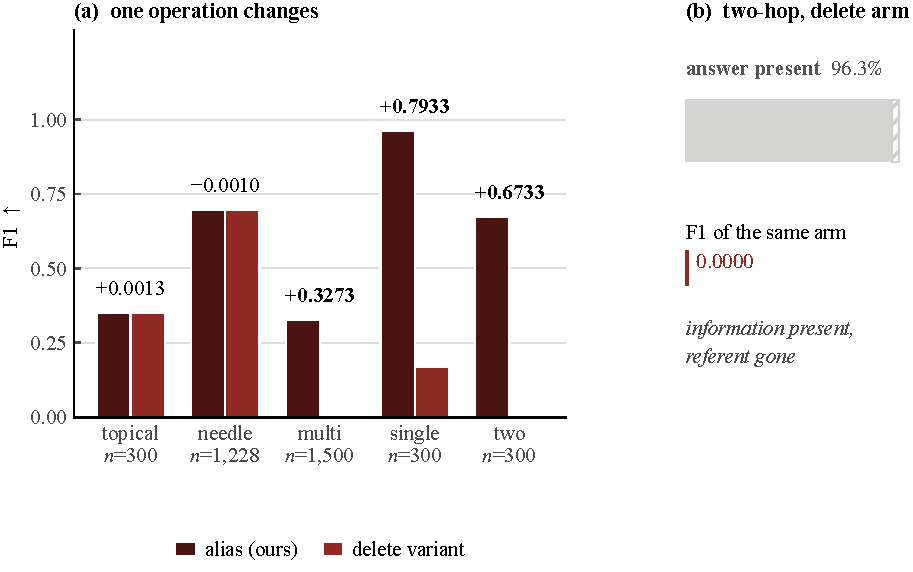
\includegraphics[width=\textwidth]{figures/fig3_alias.pdf}
\caption{Replacing the alias operation by deletion, with the context construction otherwise
unchanged, on five settings. (a) The difference concentrates exactly where the anchor is a
protected value and vanishes where it is not; labels give the paired difference of the two
bars and a star marks an interval that excludes zero. (b) Distribution of the paired per-case
difference for the three settings where the operation matters. The mass sits at both ends
because a case is either answered or not, and the mean gain is largest on the single-hop
variant. (c) In the two-hop variant the answer is still in the prompt after $96.3\%$ of the
deletions, and F1 is zero.}
\label{fig:aliasdelete}
\end{figure*}

% Fig.6 —— 两个真实案例的定性对比（预测为模型实际输出）
\definecolor{anchorbg}{HTML}{DCE4E6}
\definecolor{failbg}{HTML}{F0E4E2}
\definecolor{okbg}{HTML}{E4EAE7}

\begin{figure*}[t]
\centering

\begin{minipage}[t]{0.47\textwidth}
\centering
{\small\bfseries (a) two-hop: the answer sits behind a chain}\\[3pt]
{\scriptsize\itshape Q: which device does account \texttt{ACCT-5f31} operate?}\\[4pt]
\begin{flushleft}\ttfamily\scriptsize\setlength{\parskip}{1.5pt}
\textcolor{black!45}{164}\ \ \colorbox{anchorbg}{\strut account ACCT-5f31} belongs to \colorbox{anchorbg}{\strut user U-5a675c}\\
\textcolor{black!45}{\dots}\\
\textcolor{black!45}{170}\ \ \colorbox{anchorbg}{\strut user U-5a675c} operates device \underline{sensor\_422708\_15}
\end{flushleft}
\vspace{3pt}
{\scriptsize\itshape after aliasing, both links keep a name:}\\[3pt]
\begin{flushleft}\ttfamily\scriptsize
\colorbox{anchorbg}{\strut account [ACCT-A]} belongs to \colorbox{anchorbg}{\strut user [USER-B]}\\
\colorbox{anchorbg}{\strut user [USER-B]} operates device \underline{sensor\_422708\_15}
\end{flushleft}
\end{minipage}\hfill
\begin{minipage}[t]{0.47\textwidth}
\centering
{\small\bfseries (b) multi-entity: the answer looks like a distractor}\\[3pt]
{\scriptsize\itshape Q: which persona id is recorded for account \texttt{ACCT-447f...}?}\\[4pt]
\begin{flushleft}\ttfamily\scriptsize\setlength{\parskip}{1.5pt}
\textcolor{black!45}{07}\ \ \{``device'': ``dehumidifiers'',\\
\phantom{07}\ \ \ ``id'': \underline{``multi\_0166\_00''}, \dots\}\\
\textcolor{black!45}{08}\ \ Private contact record:\\
\textcolor{black!45}{09}\ \ Contact email: contact.e67e...\\
\textcolor{black!45}{11}\ \ \colorbox{anchorbg}{\strut Account ID: ACCT-447fa54ac66d}
\end{flushleft}
\vspace{3pt}
{\scriptsize\itshape the target account is the eleventh of sixteen,}\\
{\scriptsize\itshape and its record is shaped like every other record.}
\end{minipage}

\vspace{7pt}
\resizebox{\textwidth}{!}{%
\begin{tabular}{lcccc}
\toprule
 & \arm{full} & \arm{alias} & \arm{delete} & \textsc{DARK} \\
\midrule
(a)\ \ two-hop, \texttt{lbc-hotpotqa-0000} & \colorbox{okbg}{sensor\_422708\_15} & \colorbox{okbg}{sensor\_422708\_15} & \colorbox{failbg}{UNKNOWN} & \colorbox{okbg}{sensor\_422708\_15} \\
(b)\ \ multi-entity, \texttt{multi-0032} & \colorbox{failbg}{UNKNOWN} & \colorbox{okbg}{multi\_0166\_00} & \colorbox{failbg}{UNKNOWN} & \colorbox{okbg}{multi\_0166\_00} \\
\bottomrule
\end{tabular}}

\caption{Two cases where the routing changes the answer, with the predictions the reader
actually produced. In (a) the question names an account that reaches the answer only through
a user identifier six records later; deleting either link leaves the answer present but
unreachable, and the model returns \textsc{unknown}. In (b) the answer sits in one of sixteen
near-identical account records, so the uncompressed prompt \emph{also} fails---here the
distractor structure, not the budget, is what defeats the reader---while both aliasing arms
answer correctly. Shaded spans mark the names that keep a chain addressable.}
\label{fig:cases}
\end{figure*}


Figure~\ref{fig:cases} shows the two failure modes at the level of a single case, with the
predictions the reader actually produced.

The two-hop column is the most informative single result in this paper. Under the delete
variant the reference answer is present in the context in $96.3\%$ of cases, so GIC is
essentially saturated, and F1 is $0.0000$. The information is in the prompt; the reader
cannot use it, because the identifier saying which record it belongs to has been removed.
String-presence metrics do not detect this failure, which is why we report task quality and
leakage as separate endpoints rather than as one utility score.

\subsection{Question-side aliasing}

Aliasing the context without rewriting the question produces a prompt whose halves use
different names for the same entity. On the 112-case set we measured both settings with the
pipeline otherwise unchanged: \arm{alias} moves from $0.4933$ to $0.6719$ ($+0.1786$) and
\arm{alias\_budget\_link} from $0.5048$ to $0.7450$ ($+0.2402$). The step costs nothing in
privacy, since both halves stay free of the raw value, and it is the difference between a
prompt the reader can use and one it cannot. We therefore treat the pair $(q',P)$ rather
than $P$ alone as the object of study, and verify the mapping before generation.

\subsection{The direction of the refill traversal}

Section~\ref{sec:method-budget} noted that the traversal direction for refill units is an
empirical choice. We ran both variants end to end.

\begin{center}\small
\setlength{\tabcolsep}{4pt}
\resizebox{\columnwidth}{!}{%
\begin{tabular}{lcccc}
\toprule
Benchmark & increasing & decreasing & $\Delta$ & 95\% CI \\
\midrule
extension ($2{,}728$) & 0.4937 & 0.4832 & $-0.0106$ & $[-0.028,+0.007]$ \\
main set ($112$)      & 0.6366 & 0.5844 & $-0.0522$ & $[-0.124,+0.019]$ \\
topical ($300$)       & 0.3516 & 0.3172 & $-0.0344$ & $[-0.090,+0.020]$ \\
single-hop ($300$)    & 0.9607 & 0.9719 & $+0.0111$ & $[-0.008,+0.032]$ \\
two-hop ($300$)       & 0.6733 & 0.0167 & $-0.6567$ & $[-0.712,-0.599]$ \\
\bottomrule
\end{tabular}}
\end{center}

For four of the five rows the interval includes zero. Only the two-hop benchmark separates
the two variants, and it separates them completely. There the answer sits six sentences from
the anchor, outside the fallback window, so whether the answer is present at all is decided
by the refill order; keeping repetitive units happens to retrieve it. We report this as what
it is: an empirical regularity of this data, consistent with the anti-correlation measured at
the start of this section, but not a principled guarantee. The principled remedy is to widen
the relevant region until it covers the answer, which Section~\ref{sec:discussion} takes up.

\subsection{Where the rule applies}

Running the same pipeline on the three LongBench-derived variants locates the boundary.

\begin{center}\small
\setlength{\tabcolsep}{4pt}
\resizebox{\columnwidth}{!}{%
\begin{tabular}{lrrr}
\toprule
Variant & \arm{full} & \arm{alias} & \textsc{DARK} \\
\midrule
topical ($300$)     & 0.4181 & 0.4074 & 0.3516 \\
single-hop ($300$)  & 0.9889 & 0.9197 & 0.9607 \\
two-hop ($300$)     & 0.0967 & 0.7078 & 0.6733 \\
\bottomrule
\end{tabular}}
\end{center}

On the topical variant the questions name no entity, so there is nothing to route on; the
rule degenerates to global aliasing plus redundancy ordering, and it loses $0.0665$ against
the uncompressed prompt. We report that variant as out of scope, not as a success.

The two-hop row carries a second observation we did not anticipate. Without sanitization the
raw prompt scores $0.0967$; with global aliasing it scores $0.7078$. The account identifiers
in this variant are long hexadecimal strings differing in a few characters, and replacing
them with short distinct tokens makes the task \emph{easier} for the reader. Privacy and
utility move in the same direction here, which is a useful counterpoint to the usual framing
but also a reminder that the effect belongs to the identifier surface form, not to the
routing rule.
